\section{Study Design}
\label{sec:design}

% In this section, we describe the data collection process and 
% the overview of the collected dataset. 
This section describes our study design, including research questions, data collection, metrics computation, and data description.

\subsection{Research Questions}
\label{sec:rqs}

To identify the characteristics of the visual issue reports, we addressed the following three research questions, focusing on Report (RQ1), Discussion (RQ2), and Fix (RQ3). 
\begin{itemize}
	\item[RQ1:] \textbf{\RQone{}}\\
	Developers often suffer from reproducing bugs with the reported information~\citep{DBLP:conf/sigsoft/ChaparroLZMPMBN17}\citep{DBLP:conf/icsm/0001KC20}\citep{zimmermann2010TSE}. 
	On the other hands, as reporters are not always developers, it is not easy to tell what they did and what they encount~\citep{DBLP:conf/sigsoft/ChaparroBLMMPPN19}. Thus, GitHub developed a function that can easily provide information with videos and officially announced the function release on May, 2021~\citep{github-video-blog}. Potter and Faulconer~\citep{POTTER1975} showed that visual images are a more effective approach to describe what people want to communicate and let other people understand it, compared with texts. We hypothesize that videos can reduce the effort for reporting bugs. In this RQ, we measured the number of words in the description of issues as a proxy measure for the effort. 
	\item[RQ2:] \textbf{\RQtwo{}}\\
	We suppose visual issue reports provide 
	more information than the other issue reports. 
	Consequently, developers could discuss the details and 
	result in active discussions. 
	In this RQ, we clarify whether this assumption is true. 
	We measured the activity in terms of 
	the first response time, and
	the number of comments.
	%, and the number of words. 
	\item[RQ3:] \textbf{\RQthree{}}\\
	% We suppose that developers use visualization 
	% in particular issues. 
	% For example, developers may use visualization 
	% to share the way to reproduce bugs. 
	% In this RQ, we clarify the differences 
	% between the issues with and without 
	% visualization. 
	Zimmermann~\et~\citep{zimmermann2010TSE} reported that issue reports occasionally have missing or incorrect steps to reproduce bugs, which delays the entire bug-fixing process~\citep{github-video-blog}. Also, Ohira et al. ~\citep{DBLP:conf/icsm/OhiraHOM12} shows that bug-fixing activities delays when the reporter and developer are different persons because they require communications. Visual issues may mitigate this issue by facilitating their communication. In this RQ, we measure the time from reported to closed to evaluate how quickly visual issue reports are resolved, compared with issues without videos or images. 
\end{itemize}

\subsection{Context Selection}
\label{sec:design:context}
To select projects as context for our study, we employed \texttt{GHS}\citep{msr2021data}. GHS can find repositories satisfying specific criteria. To filter out unpopular, inactive repositories, or repositories that have no issues, we set up the following criteria.
\begin{itemize}
	\item the number of stars $\geq$ 10
	\item the number of issue reports $\geq$ 1
	\item at least one commit was made in 2021
\end{itemize}
Consequently, the number of the repositories satisfying the criteria was 289,115. From November 2021 to December 2021, we collected 770,656 closed issue reports from 4,173 projects that were randomly selected. While the number of sampled projects seems odds, we collected all the closed issue reports from as many projects as possible in the limited time.  
%As the sampled projects accounts for only less than 2\% of all repositories, we discuss the threat to validity of this process in \sec{sec:limitation}. 


% 
\begin{figure*}[t]
\centering
% 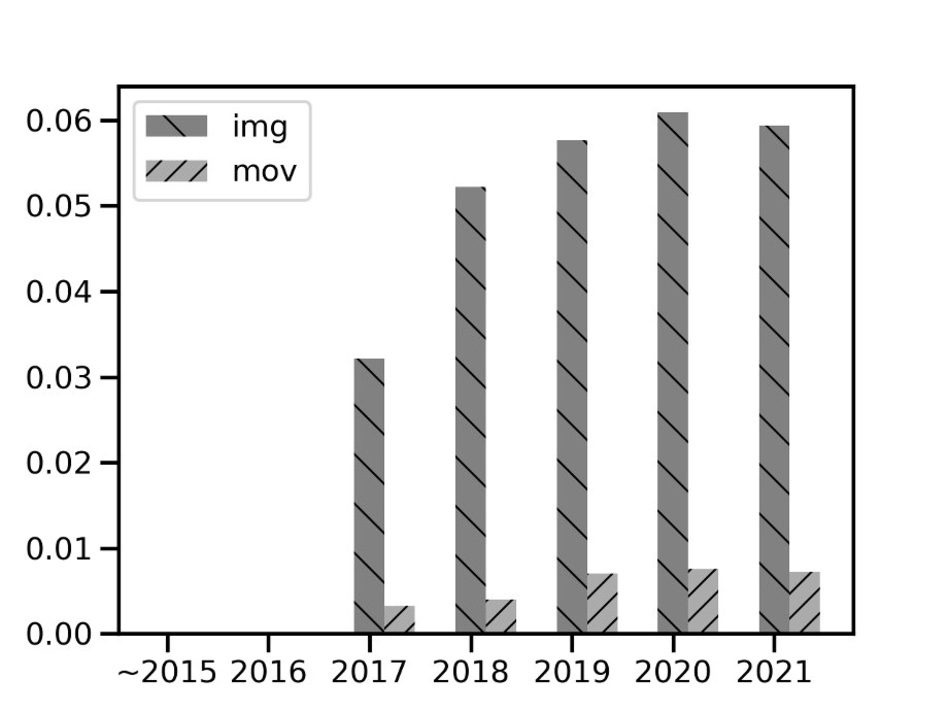
\includegraphics[width=1\linewidth]{./figures/data-category-trend.pdf}
\caption{ 
  An overview of the data collection
  }
\label{fig:data-collection-overview}
\end{figure*}


\subsection{Data Collection}
%\fig{fig:data-collection-overview} shows an overview of the data collection process. 
We first collected closed issue reports with \texttt{PyGitHub}\footnote{\url{https://pygithub.readthedocs.io/en/latest/index.html}} that internally execute GitHub API v3\footnote{\url{https://docs.github.com/en/rest}}. 
Next, we collected videos and images attached to the issue reports. While GitHub users can see videos and images on issue pages, the videos and images are stored in different URLs. As the URLs are written in the text description of issue reports, we parsed them with regular expressions and downloaded them. The regular expressions we used are shown as follows:
\begin{quote}
\addtolength\leftmargini{0in}
{\it https://user-images.githubusercontent.com/[a-zA-Z0-9\textbackslash-/]+\textbackslash.[a-zA-Z0-9]+}
\end{quote}
Each downloaded file was determined to be a image or video by its extension. Specifically, png, PNG, jpg, JPG, and jpeg are treated as images, and  gif, GIF, mp4, MP4, and mov as videos.
Consequently, we downloaded 33,079 images and 3,819 movies
with the collected URLs.\masa{to kuramoto: i wrote these numbers. are the numbers correct?} 


% \begin{table*}[h]
    \begin{center}
    \caption{Examples of the retrieved issues with the values of the attributes}
    \begin{tabular}{c c c c c c c} 
      \toprule
      \textbf{IssueCreatedYear} &
      \textbf{ResolutionTime} &
      \textbf{Images} &
      \textbf{Videos} &
      \textbf{Comments} &
      \textbf{FirstCommentTime} &
      \textbf{DescriptionLength} \\
      \midrule
      2020 & 6.99861111 & 0 & 0 & 1 & 6.99861111 & 4430\\
      2020 & 41.9594329 & 1 & 0 & 3 & 17.7784722 & 85\\
      2020 & 43.8850579 & 0 & 0 & 2 & 0.49828704 & 56\\
      2020 & 44.0935532 & 0 & 0 & 4 & 0.91277778 & 33\\
      2020 & 0.14934028 & 0 & 0 & 8 & 0.08077546 & 244\\
      2020 & 59.5670949 & 2 & 0 & 5 & 0.39472222 & 102\\
      2020 & 74.9322569 & 0 & 0 & 0 & -          & 24\\
      \bottomrule
    \end{tabular}
    \label{tab:example-dataset}
    \end{center}
  \end{table*}

% We extract a part of the retrieved issues in \tab{tab:example-dataset}. 
% Each row corresponds to the values of the attributes of an issue. 
%
\begin{table}[t]
    \begin{center}
    \caption{The attributes we collected from the issues}
    \scalebox{0.85}[0.85]{
    \begin{tabular}{ll} 
        \toprule
        \multicolumn{1}{c}{\textbf{Attributes}} & \multicolumn{1}{c}{\textbf{Description}} \\ 
        \midrule
        $IssueResolvedTime$ & The time until the issue is resolved (day) \\
        $FirstCommentTime$ & The time until the first comment (day) \\
        $\#comments$ & The number of comments \\
        $\#chars$ & \masa{im not sure what is this} \\
        $\#imgs$ & \# of attached images when the issue is created \\
        $\#movs$ & \# of attached movies when the issue is created \\
        $\#words$ &  \masa{im not sure what is this} \\
        $IssueCreatedYear$ & The year when the issue is created \\
        \bottomrule
    \end{tabular}
    }
    \label{tab:issue-attr}
    \end{center}
\end{table}


\begin{table}[t]
    \begin{center}
    \caption{The attributes we collected from the issues}
    \scalebox{0.85}[0.85]{
    \begin{tabular}{ll} 
        \toprule
        \multicolumn{1}{c}{\textbf{Attributes}} & \multicolumn{1}{c}{\textbf{Description}} \\ 
        \midrule
        $IssueResolvedTime$ & The time until the issue is resolved (day) \\
        $FirstCommentTime$ & The time until the first comment (day) \\
        $\#comments$ & The number of comments \\
        $\#chars$ & \masa{im not sure what is this} \\
        $\#imgs$ & \# of attached images when the issue is created \\
        $\#movs$ & \# of attached movies when the issue is created \\
        $\#words$ &  \masa{im not sure what is this} \\
        $IssueCreatedYear$ & The year when the issue is created \\
        \bottomrule
    \end{tabular}
    }
    \label{tab:issue-attr}
    \end{center}
\end{table}

\subsection{Analysis}
We retrieved the attributes from the collected issue reports.
\tab{tab:issue-attr} shows seven attributes extracted from 
the issue reports. 
The attributes can be classified into three dimensions, 
``Report'', ``Discussion'', and ``Fix''. 
The attributes in the dimension ``Report'' are extracted from 
the description of issue reports or attached files 
when the issue was created. 
In particular, in RQ1, we 
%calculate 
utilize the number of words 
in reports (\ie, $DescriptionLength$) for Img, Vid, and None. 
In addition,  $\#imgs$ and $\#vids$ are used to show 
dataset description. 
Note that these attributes are not calculated from either title, not comments (i.e., only descriptions were used). 
Also, when computing $DescriptionLength$, if the description of the issue report 
includes URLs for images/videos, 
we exclude them from the description because these are not words.

The dimension ``Discussion'' has two attributes, $Comments$ and $FirstCommentTime$. $Comments$ is the number of comments were made in the issue report. We utilize this attribute as a proxy measure of discussion effort. $FirstCommentTime$ is the days subtract from when the first comment was made to when issue was reported. We employ this attribute for measuring developers' interest. 

The dimension ``Fix'' has one attribute $IssueResolvedTime$ which shows the time from reported to fixed. 
Note that some negative values of $IssueResolvedTime$ were observed. We investigated it manually and found that these are because of a bug in GitHub.  We excluded those issues that have negative values from our dataset. 
In addition, we excluded issue reports resolved in too short or long periods (e.g., 30 seconds) because they might be issued after being fixed or might not be fixed in reality.
%\kashiwa{check please}
Specifically, we only use the issue reports that meet the condition: $30\ sec \leq IssueResolvedTime \leq 1\ year$.
The number of issue reports that meet this condition is 711,160 (92.23\%).


\kashiwa{Write what do you analyze (e.g., compare them in median)}
To evaluate the difference, we used a non-parametric test \textit{Steel-Dwass test}.
\kashiwa{Write what this test is}
\kashiwa{Write why this test is selected}
because our preliminary study shows that 
the distributions for each category do not 
come from normal distributions.
\kashiwa{Write the reason why correction is not needed (i.e., how to deal with family-wise error rate)}
